% network: M-to-N circuit with 4 rectangular components T1..T4; top branch T1, middle T2-T3, bottom branch T4.
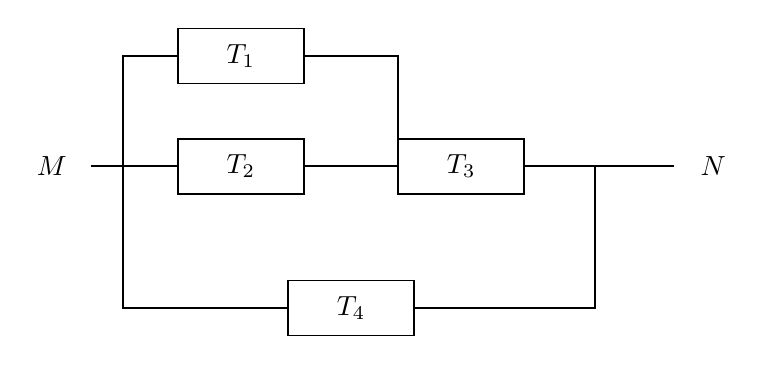
\begin{tikzpicture}[line width=.6pt,font=\normalsize,
  comp/.style={rectangle,draw,fill=white,minimum width=16mm,minimum height=7mm,inner sep=1pt}]
  \node[comp] (T1) at (2.4,2.6) {$T_{1}$};
  \node[comp] (T2) at (2.4,1.2) {$T_{2}$};
  \node[comp] (T3) at (5.2,1.2) {$T_{3}$};
  \node[comp] (T4) at (3.8,-0.6) {$T_{4}$};
  \node at (0,1.2) {$M$};
  \node at (8.4,1.2) {$N$};
  % main line M-T2-T3-N
  \draw (0.5,1.2) -- (T2.west);
  \draw (T2.east) -- (T3.west);
  \draw (T3.east) -- (7.9,1.2);
  % upper branch through T1: from main line up, across, back down to T2-T3 middle
  \draw (0.9,1.2) -- (0.9,2.6) -- (T1.west);
  \draw (T1.east) -- (4.4,2.6) -- (4.4,1.2);
  % lower branch through T4: from main line down/around, across, back up to N line
  \draw (0.9,1.2) -- (0.9,-0.6) -- (T4.west);
  \draw (T4.east) -- (6.9,-0.6) -- (6.9,1.2);
\end{tikzpicture}
